% Options for packages loaded elsewhere
\PassOptionsToPackage{unicode}{hyperref}
\PassOptionsToPackage{hyphens}{url}
\PassOptionsToPackage{dvipsnames,svgnames,x11names}{xcolor}
%
\documentclass[
  letterpaper,
  DIV=11,
  numbers=noendperiod]{scrartcl}

\usepackage{amsmath,amssymb}
\usepackage{iftex}
\ifPDFTeX
  \usepackage[T1]{fontenc}
  \usepackage[utf8]{inputenc}
  \usepackage{textcomp} % provide euro and other symbols
\else % if luatex or xetex
  \usepackage{unicode-math}
  \defaultfontfeatures{Scale=MatchLowercase}
  \defaultfontfeatures[\rmfamily]{Ligatures=TeX,Scale=1}
\fi
\usepackage{lmodern}
\ifPDFTeX\else  
    % xetex/luatex font selection
\fi
% Use upquote if available, for straight quotes in verbatim environments
\IfFileExists{upquote.sty}{\usepackage{upquote}}{}
\IfFileExists{microtype.sty}{% use microtype if available
  \usepackage[]{microtype}
  \UseMicrotypeSet[protrusion]{basicmath} % disable protrusion for tt fonts
}{}
\makeatletter
\@ifundefined{KOMAClassName}{% if non-KOMA class
  \IfFileExists{parskip.sty}{%
    \usepackage{parskip}
  }{% else
    \setlength{\parindent}{0pt}
    \setlength{\parskip}{6pt plus 2pt minus 1pt}}
}{% if KOMA class
  \KOMAoptions{parskip=half}}
\makeatother
\usepackage{xcolor}
\setlength{\emergencystretch}{3em} % prevent overfull lines
\setcounter{secnumdepth}{-\maxdimen} % remove section numbering
% Make \paragraph and \subparagraph free-standing
\makeatletter
\ifx\paragraph\undefined\else
  \let\oldparagraph\paragraph
  \renewcommand{\paragraph}{
    \@ifstar
      \xxxParagraphStar
      \xxxParagraphNoStar
  }
  \newcommand{\xxxParagraphStar}[1]{\oldparagraph*{#1}\mbox{}}
  \newcommand{\xxxParagraphNoStar}[1]{\oldparagraph{#1}\mbox{}}
\fi
\ifx\subparagraph\undefined\else
  \let\oldsubparagraph\subparagraph
  \renewcommand{\subparagraph}{
    \@ifstar
      \xxxSubParagraphStar
      \xxxSubParagraphNoStar
  }
  \newcommand{\xxxSubParagraphStar}[1]{\oldsubparagraph*{#1}\mbox{}}
  \newcommand{\xxxSubParagraphNoStar}[1]{\oldsubparagraph{#1}\mbox{}}
\fi
\makeatother

\usepackage{color}
\usepackage{fancyvrb}
\newcommand{\VerbBar}{|}
\newcommand{\VERB}{\Verb[commandchars=\\\{\}]}
\DefineVerbatimEnvironment{Highlighting}{Verbatim}{commandchars=\\\{\}}
% Add ',fontsize=\small' for more characters per line
\usepackage{framed}
\definecolor{shadecolor}{RGB}{241,243,245}
\newenvironment{Shaded}{\begin{snugshade}}{\end{snugshade}}
\newcommand{\AlertTok}[1]{\textcolor[rgb]{0.68,0.00,0.00}{#1}}
\newcommand{\AnnotationTok}[1]{\textcolor[rgb]{0.37,0.37,0.37}{#1}}
\newcommand{\AttributeTok}[1]{\textcolor[rgb]{0.40,0.45,0.13}{#1}}
\newcommand{\BaseNTok}[1]{\textcolor[rgb]{0.68,0.00,0.00}{#1}}
\newcommand{\BuiltInTok}[1]{\textcolor[rgb]{0.00,0.23,0.31}{#1}}
\newcommand{\CharTok}[1]{\textcolor[rgb]{0.13,0.47,0.30}{#1}}
\newcommand{\CommentTok}[1]{\textcolor[rgb]{0.37,0.37,0.37}{#1}}
\newcommand{\CommentVarTok}[1]{\textcolor[rgb]{0.37,0.37,0.37}{\textit{#1}}}
\newcommand{\ConstantTok}[1]{\textcolor[rgb]{0.56,0.35,0.01}{#1}}
\newcommand{\ControlFlowTok}[1]{\textcolor[rgb]{0.00,0.23,0.31}{\textbf{#1}}}
\newcommand{\DataTypeTok}[1]{\textcolor[rgb]{0.68,0.00,0.00}{#1}}
\newcommand{\DecValTok}[1]{\textcolor[rgb]{0.68,0.00,0.00}{#1}}
\newcommand{\DocumentationTok}[1]{\textcolor[rgb]{0.37,0.37,0.37}{\textit{#1}}}
\newcommand{\ErrorTok}[1]{\textcolor[rgb]{0.68,0.00,0.00}{#1}}
\newcommand{\ExtensionTok}[1]{\textcolor[rgb]{0.00,0.23,0.31}{#1}}
\newcommand{\FloatTok}[1]{\textcolor[rgb]{0.68,0.00,0.00}{#1}}
\newcommand{\FunctionTok}[1]{\textcolor[rgb]{0.28,0.35,0.67}{#1}}
\newcommand{\ImportTok}[1]{\textcolor[rgb]{0.00,0.46,0.62}{#1}}
\newcommand{\InformationTok}[1]{\textcolor[rgb]{0.37,0.37,0.37}{#1}}
\newcommand{\KeywordTok}[1]{\textcolor[rgb]{0.00,0.23,0.31}{\textbf{#1}}}
\newcommand{\NormalTok}[1]{\textcolor[rgb]{0.00,0.23,0.31}{#1}}
\newcommand{\OperatorTok}[1]{\textcolor[rgb]{0.37,0.37,0.37}{#1}}
\newcommand{\OtherTok}[1]{\textcolor[rgb]{0.00,0.23,0.31}{#1}}
\newcommand{\PreprocessorTok}[1]{\textcolor[rgb]{0.68,0.00,0.00}{#1}}
\newcommand{\RegionMarkerTok}[1]{\textcolor[rgb]{0.00,0.23,0.31}{#1}}
\newcommand{\SpecialCharTok}[1]{\textcolor[rgb]{0.37,0.37,0.37}{#1}}
\newcommand{\SpecialStringTok}[1]{\textcolor[rgb]{0.13,0.47,0.30}{#1}}
\newcommand{\StringTok}[1]{\textcolor[rgb]{0.13,0.47,0.30}{#1}}
\newcommand{\VariableTok}[1]{\textcolor[rgb]{0.07,0.07,0.07}{#1}}
\newcommand{\VerbatimStringTok}[1]{\textcolor[rgb]{0.13,0.47,0.30}{#1}}
\newcommand{\WarningTok}[1]{\textcolor[rgb]{0.37,0.37,0.37}{\textit{#1}}}

\providecommand{\tightlist}{%
  \setlength{\itemsep}{0pt}\setlength{\parskip}{0pt}}\usepackage{longtable,booktabs,array}
\usepackage{calc} % for calculating minipage widths
% Correct order of tables after \paragraph or \subparagraph
\usepackage{etoolbox}
\makeatletter
\patchcmd\longtable{\par}{\if@noskipsec\mbox{}\fi\par}{}{}
\makeatother
% Allow footnotes in longtable head/foot
\IfFileExists{footnotehyper.sty}{\usepackage{footnotehyper}}{\usepackage{footnote}}
\makesavenoteenv{longtable}
\usepackage{graphicx}
\makeatletter
\def\maxwidth{\ifdim\Gin@nat@width>\linewidth\linewidth\else\Gin@nat@width\fi}
\def\maxheight{\ifdim\Gin@nat@height>\textheight\textheight\else\Gin@nat@height\fi}
\makeatother
% Scale images if necessary, so that they will not overflow the page
% margins by default, and it is still possible to overwrite the defaults
% using explicit options in \includegraphics[width, height, ...]{}
\setkeys{Gin}{width=\maxwidth,height=\maxheight,keepaspectratio}
% Set default figure placement to htbp
\makeatletter
\def\fps@figure{htbp}
\makeatother

\KOMAoption{captions}{tableheading}
\makeatletter
\@ifpackageloaded{caption}{}{\usepackage{caption}}
\AtBeginDocument{%
\ifdefined\contentsname
  \renewcommand*\contentsname{Table of contents}
\else
  \newcommand\contentsname{Table of contents}
\fi
\ifdefined\listfigurename
  \renewcommand*\listfigurename{List of Figures}
\else
  \newcommand\listfigurename{List of Figures}
\fi
\ifdefined\listtablename
  \renewcommand*\listtablename{List of Tables}
\else
  \newcommand\listtablename{List of Tables}
\fi
\ifdefined\figurename
  \renewcommand*\figurename{Figure}
\else
  \newcommand\figurename{Figure}
\fi
\ifdefined\tablename
  \renewcommand*\tablename{Table}
\else
  \newcommand\tablename{Table}
\fi
}
\@ifpackageloaded{float}{}{\usepackage{float}}
\floatstyle{ruled}
\@ifundefined{c@chapter}{\newfloat{codelisting}{h}{lop}}{\newfloat{codelisting}{h}{lop}[chapter]}
\floatname{codelisting}{Listing}
\newcommand*\listoflistings{\listof{codelisting}{List of Listings}}
\makeatother
\makeatletter
\makeatother
\makeatletter
\@ifpackageloaded{caption}{}{\usepackage{caption}}
\@ifpackageloaded{subcaption}{}{\usepackage{subcaption}}
\makeatother

\ifLuaTeX
  \usepackage{selnolig}  % disable illegal ligatures
\fi
\usepackage{bookmark}

\IfFileExists{xurl.sty}{\usepackage{xurl}}{} % add URL line breaks if available
\urlstyle{same} % disable monospaced font for URLs
\hypersetup{
  pdftitle={Individual Assignment 1, International Climate Policy},
  colorlinks=true,
  linkcolor={blue},
  filecolor={Maroon},
  citecolor={Blue},
  urlcolor={Blue},
  pdfcreator={LaTeX via pandoc}}


\title{Individual Assignment 1, International Climate Policy}
\author{}
\date{}

\begin{document}
\maketitle


\begin{itemize}
\item
  Neil Stein, 12410247
\item
  \href{https://github.com/neil-stein/Assignment-1_ICP.git}{Github URL}
\end{itemize}

\begin{Shaded}
\begin{Highlighting}[]
\CommentTok{\# Setup steps}
\ImportTok{import}\NormalTok{ matplotlib.pyplot }\ImportTok{as}\NormalTok{ plt}
\ImportTok{import}\NormalTok{ seaborn }\ImportTok{as}\NormalTok{ sns}
\ImportTok{import}\NormalTok{ pandas }\ImportTok{as}\NormalTok{ pd}
\ImportTok{import}\NormalTok{ numpy }\ImportTok{as}\NormalTok{ np}
\ImportTok{import}\NormalTok{ geopandas}
\ImportTok{import}\NormalTok{ warnings}
\ImportTok{import}\NormalTok{ scipy}
\ImportTok{import}\NormalTok{ time}

\NormalTok{warnings.filterwarnings(}\StringTok{"ignore"}\NormalTok{)}

\CommentTok{\# data loading}
\NormalTok{perth\_df }\OperatorTok{=}\NormalTok{ pd.read\_csv(}\StringTok{"indiv1\_perth\_airport.csv"}\NormalTok{)}
\NormalTok{gmst\_df }\OperatorTok{=}\NormalTok{ pd.read\_csv(}\StringTok{"indiv1\_gmst\_monthly\_fixed.csv"}\NormalTok{)}
\NormalTok{us\_income\_df }\OperatorTok{=}\NormalTok{ pd.read\_csv(}\StringTok{"indiv1\_us\_counties\_incomes.csv"}\NormalTok{)}
\NormalTok{us\_temp\_df }\OperatorTok{=}\NormalTok{ pd.read\_csv(}\StringTok{"indiv1\_us\_counties\_temperature.csv"}\NormalTok{)}
\end{Highlighting}
\end{Shaded}

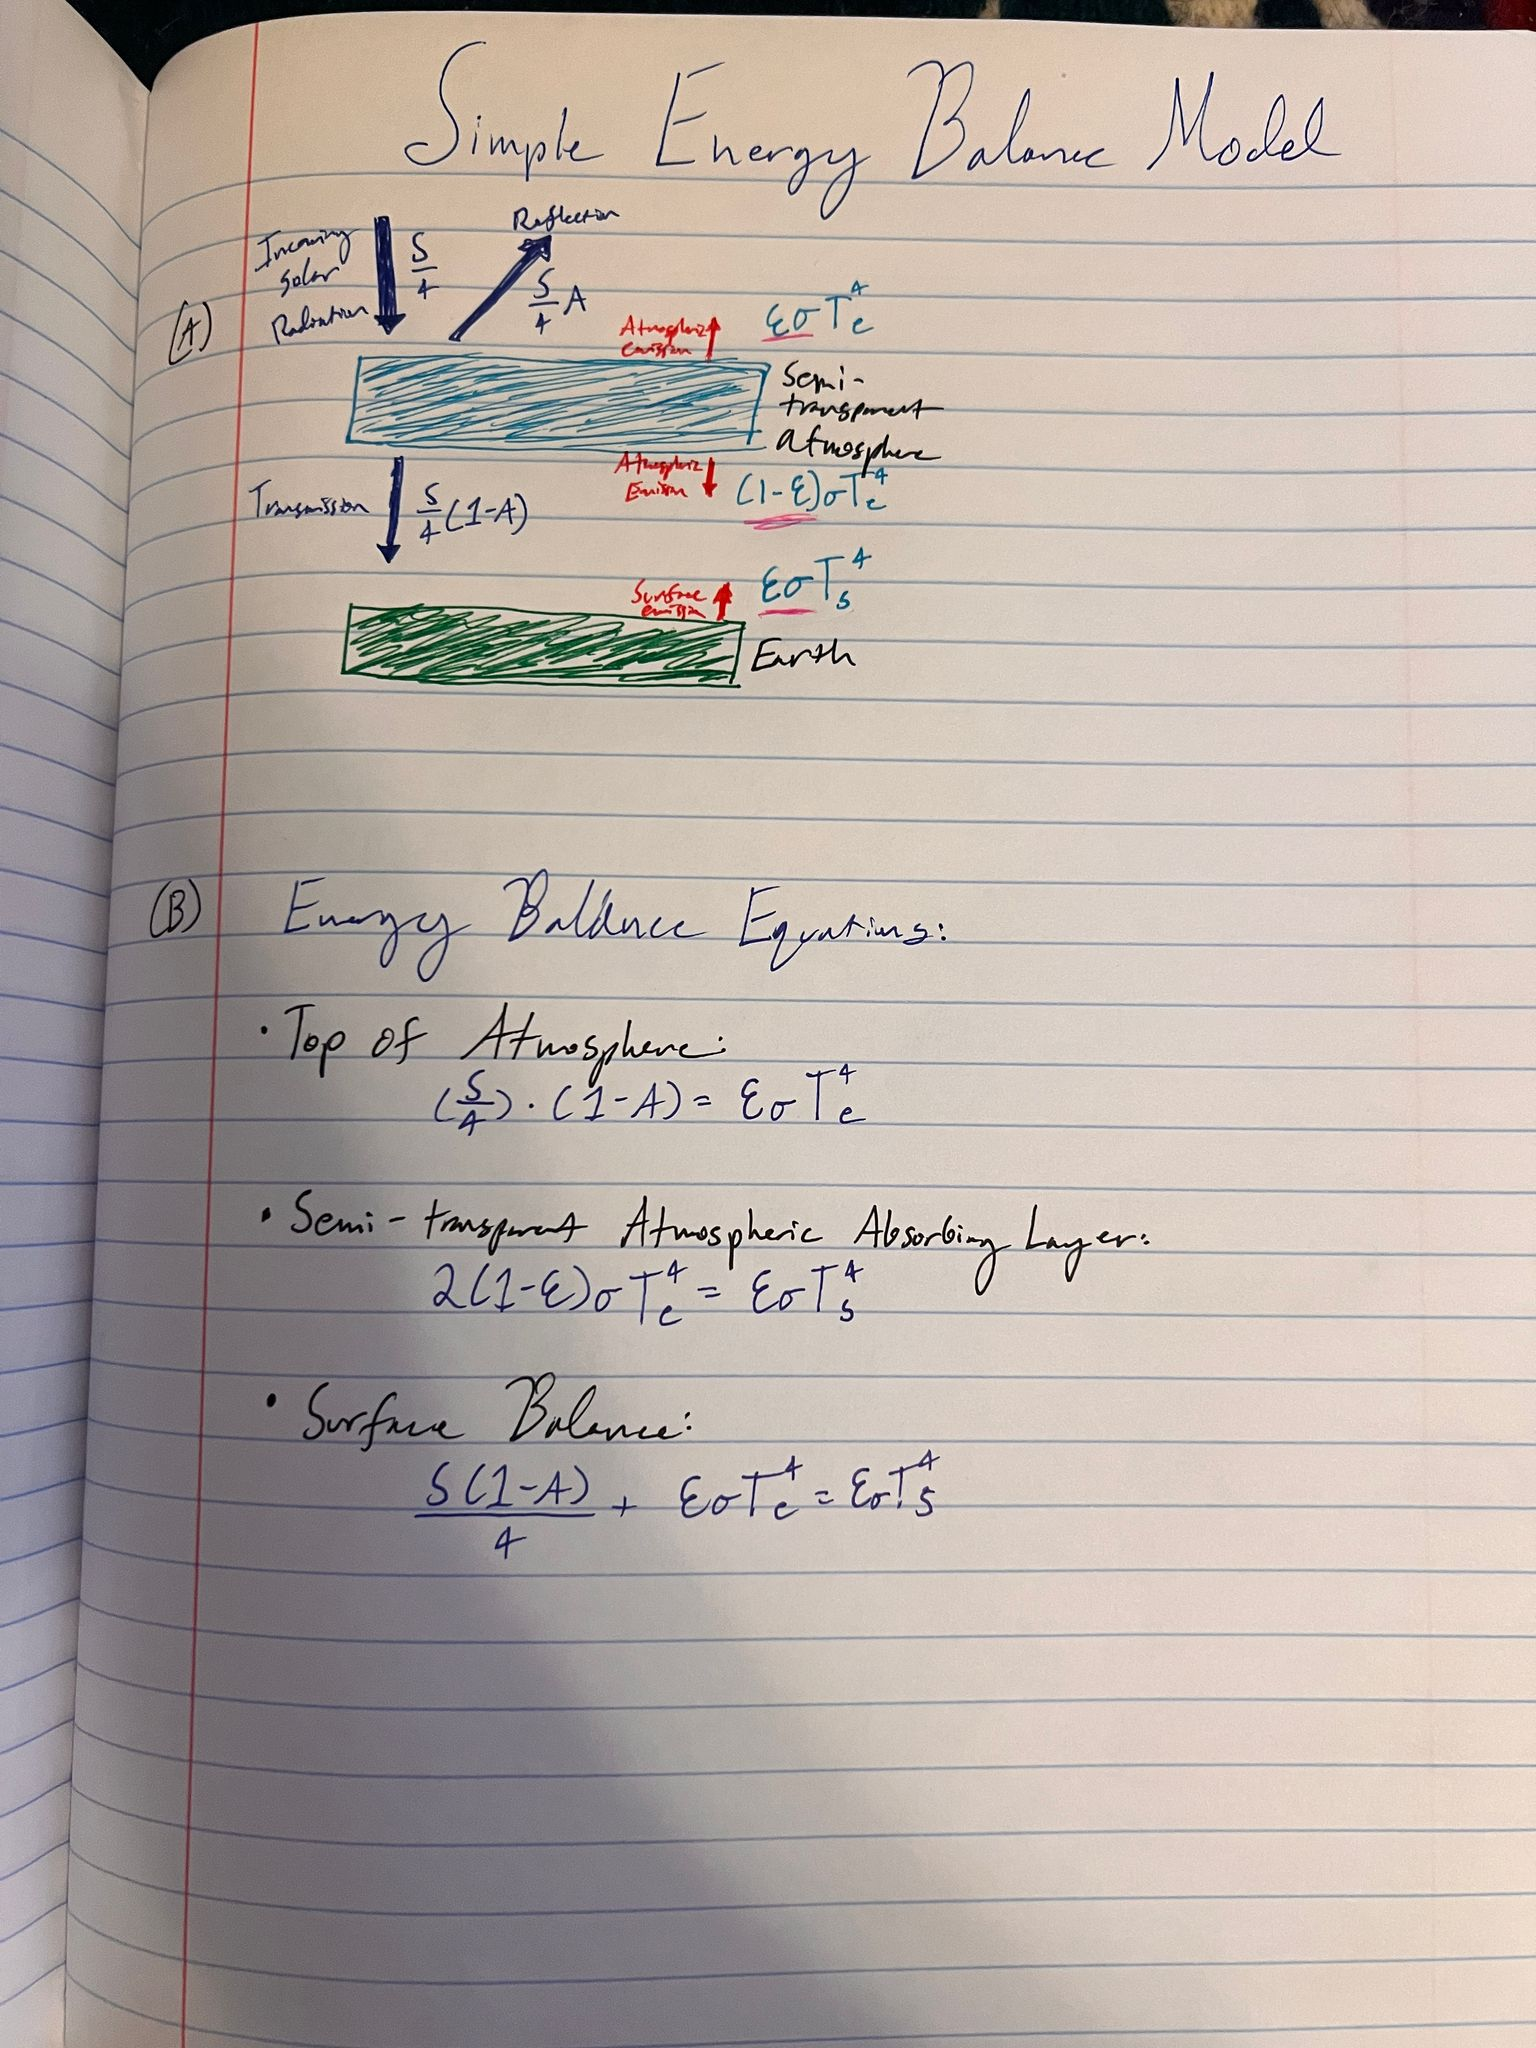
\includegraphics{Part_1_Images/parta_b.jpeg}
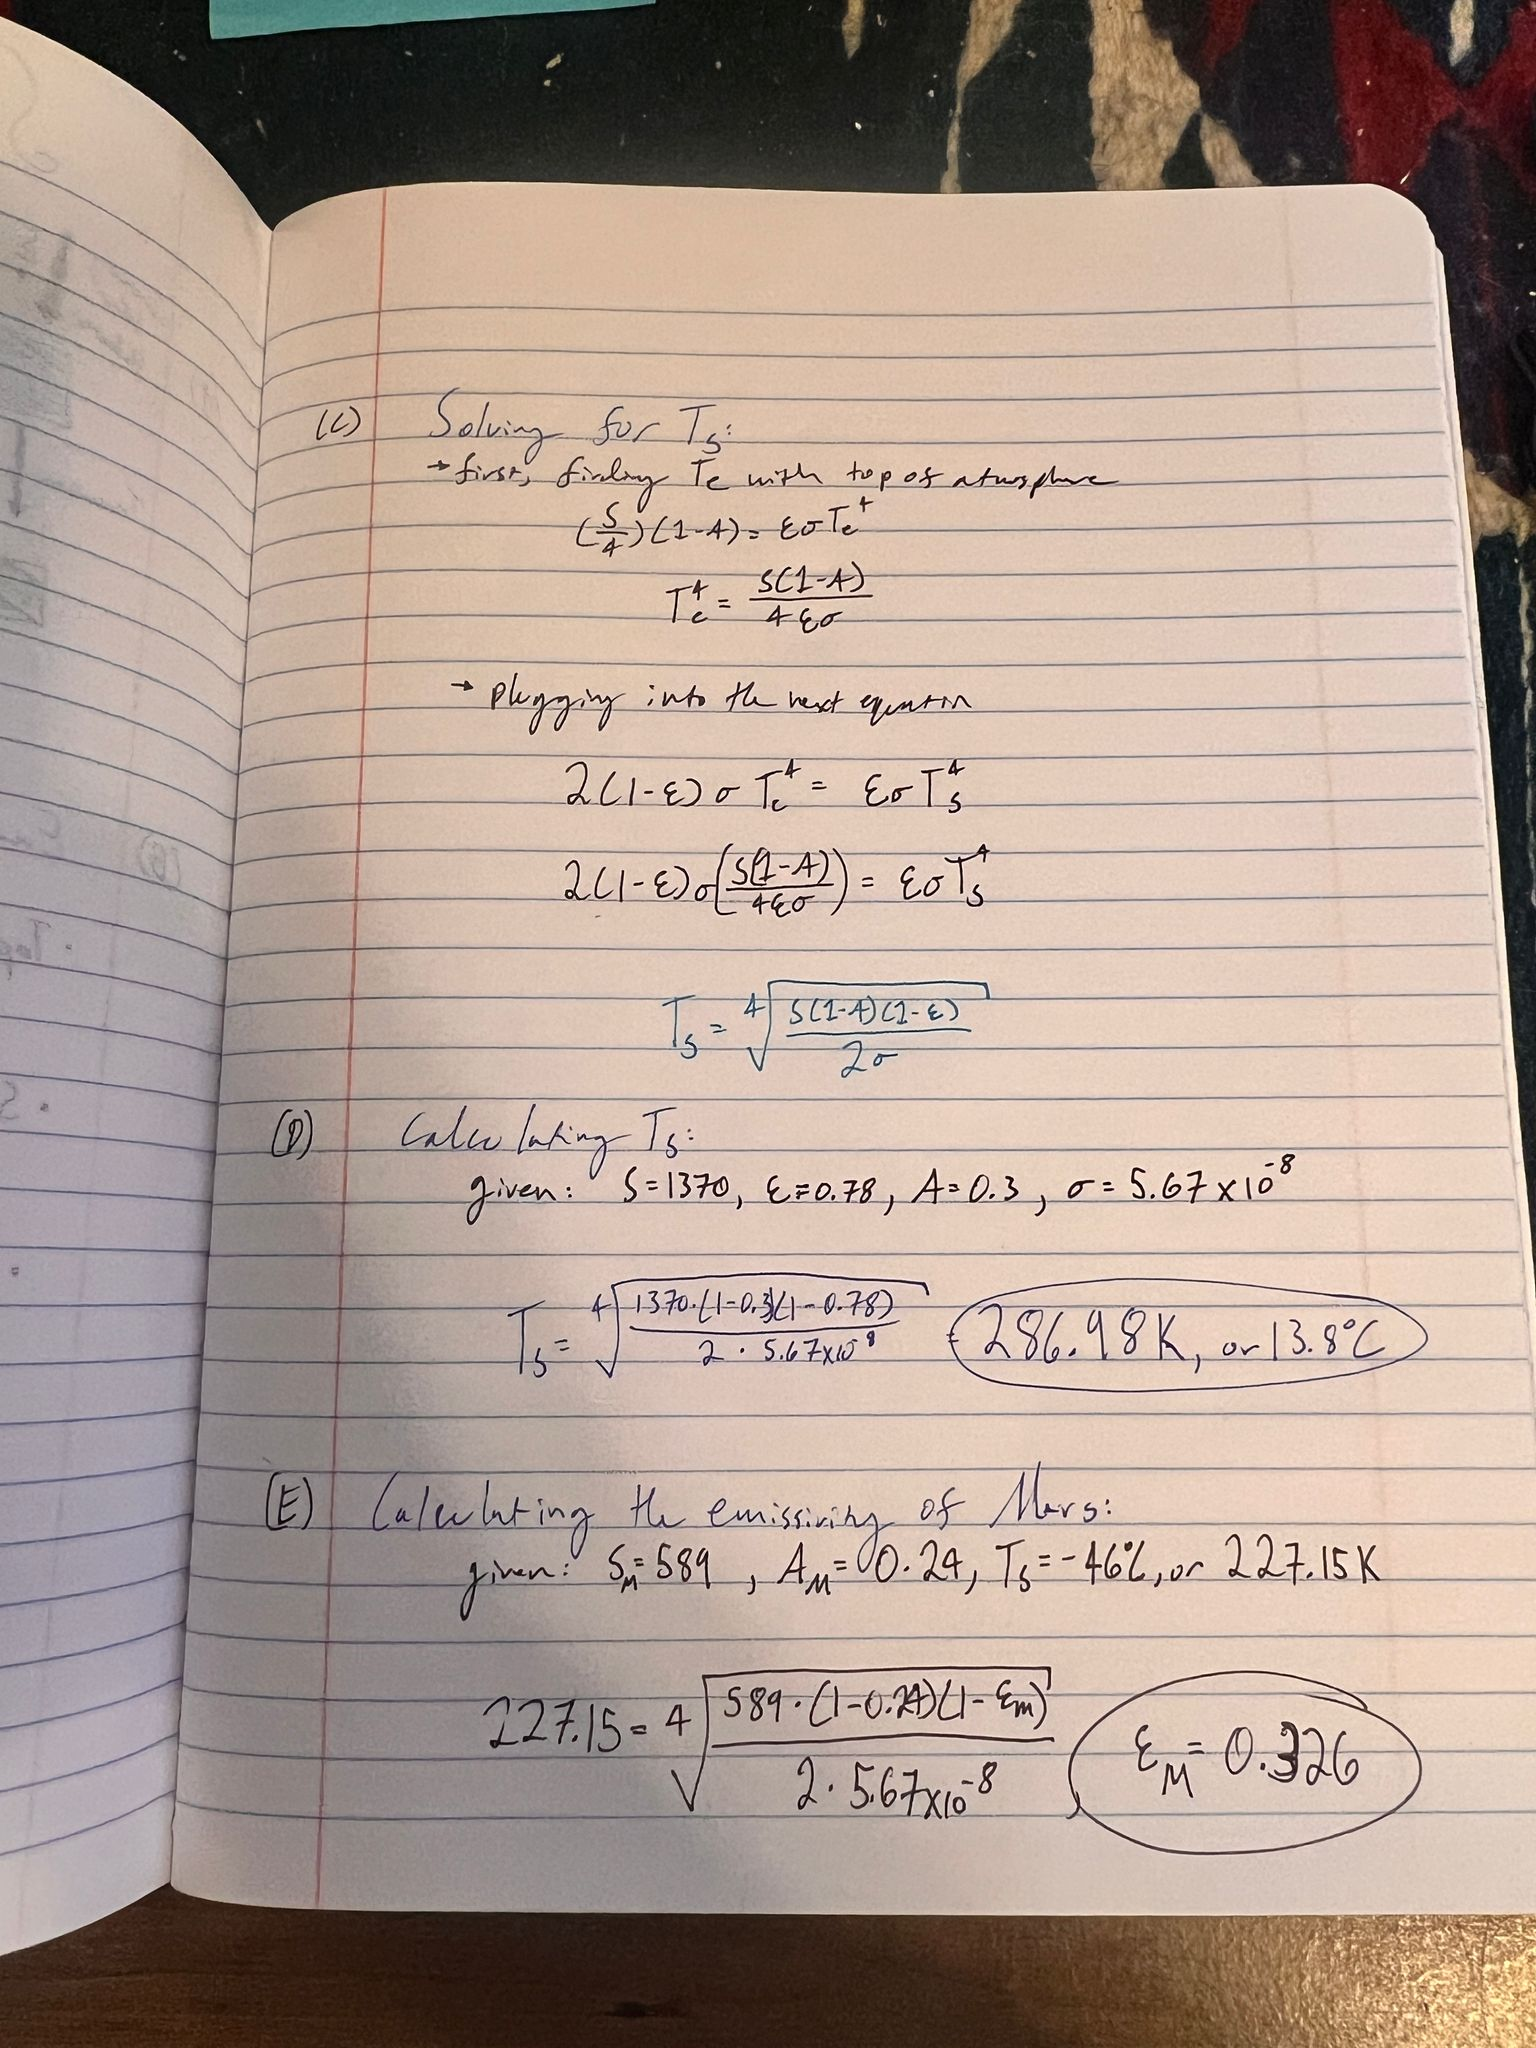
\includegraphics{Part_1_Images/partc_e.jpeg}

\begin{Shaded}
\begin{Highlighting}[]
\CommentTok{\# Problem 2 {-} Perth}
\CommentTok{\# part(a) {-} Plotting monthly precipitation}

\CommentTok{\# cleanup and reorienting the data to be grouped by month}
\NormalTok{perth\_df }\OperatorTok{=}\NormalTok{ perth\_df.dropna()}
\NormalTok{perth\_df[}\StringTok{\textquotesingle{}DATE\textquotesingle{}}\NormalTok{] }\OperatorTok{=}\NormalTok{ pd.to\_datetime(perth\_df[}\StringTok{\textquotesingle{}DATE\textquotesingle{}}\NormalTok{], }\BuiltInTok{format}\OperatorTok{=} \StringTok{\textquotesingle{}\%Y{-}\%m\textquotesingle{}}\NormalTok{)}
\NormalTok{perth\_df[}\StringTok{\textquotesingle{}MONTH\textquotesingle{}}\NormalTok{] }\OperatorTok{=}\NormalTok{ perth\_df[}\StringTok{\textquotesingle{}DATE\textquotesingle{}}\NormalTok{].dt.month}
\CommentTok{\# for future steps!}
\NormalTok{perth\_df[}\StringTok{\textquotesingle{}YEAR\textquotesingle{}}\NormalTok{] }\OperatorTok{=}\NormalTok{ perth\_df[}\StringTok{\textquotesingle{}DATE\textquotesingle{}}\NormalTok{].dt.year}

\CommentTok{\# subset the data to get 1981 {-} 2010}
\NormalTok{start\_date }\OperatorTok{=}\NormalTok{ pd.to\_datetime(}\StringTok{\textquotesingle{}1981{-}01{-}01\textquotesingle{}}\NormalTok{)}
\NormalTok{end\_date }\OperatorTok{=}\NormalTok{ pd.to\_datetime(}\StringTok{\textquotesingle{}2010{-}12{-}31\textquotesingle{}}\NormalTok{)}
\NormalTok{filtered\_perth\_df }\OperatorTok{=}\NormalTok{ perth\_df[(perth\_df[}\StringTok{\textquotesingle{}DATE\textquotesingle{}}\NormalTok{] }\OperatorTok{\textgreater{}=}\NormalTok{ start\_date) }\OperatorTok{\&}\NormalTok{ (perth\_df[}\StringTok{\textquotesingle{}DATE\textquotesingle{}}\NormalTok{] }\OperatorTok{\textless{}=}\NormalTok{ end\_date)]}

\CommentTok{\# creating our monthly averages}
\NormalTok{perth\_monthly }\OperatorTok{=}\NormalTok{ perth\_df.groupby(}\StringTok{\textquotesingle{}MONTH\textquotesingle{}}\NormalTok{)[}\StringTok{\textquotesingle{}PRCP\textquotesingle{}}\NormalTok{].mean()}


\CommentTok{\# setting up the plotting}
\NormalTok{months }\OperatorTok{=}\NormalTok{ [}\StringTok{\textquotesingle{}Jan\textquotesingle{}}\NormalTok{, }\StringTok{\textquotesingle{}Feb\textquotesingle{}}\NormalTok{, }\StringTok{\textquotesingle{}Mar\textquotesingle{}}\NormalTok{, }\StringTok{\textquotesingle{}Apr\textquotesingle{}}\NormalTok{, }\StringTok{\textquotesingle{}May\textquotesingle{}}\NormalTok{, }\StringTok{\textquotesingle{}Jun\textquotesingle{}}\NormalTok{, }\StringTok{\textquotesingle{}Jul\textquotesingle{}}\NormalTok{, }\StringTok{\textquotesingle{}Aug\textquotesingle{}}\NormalTok{, }\StringTok{\textquotesingle{}Sep\textquotesingle{}}\NormalTok{, }\StringTok{\textquotesingle{}Oct\textquotesingle{}}\NormalTok{, }\StringTok{\textquotesingle{}Nov\textquotesingle{}}\NormalTok{, }\StringTok{\textquotesingle{}Dec\textquotesingle{}}\NormalTok{]}

\NormalTok{plt.bar(months, perth\_monthly.values)}
\NormalTok{plt.xlabel(}\StringTok{"Month"}\NormalTok{)}
\NormalTok{plt.ylabel(}\StringTok{"Average Rainfall (in mm)"}\NormalTok{)}
\NormalTok{plt.title(}\StringTok{"Monthly Average Rainfall For Perth (Across 1981{-}2010)"}\NormalTok{)}
\NormalTok{plt.xticks(rotation}\OperatorTok{=}\DecValTok{45}\NormalTok{)}
\NormalTok{plt.tight\_layout()}
\NormalTok{plt.show()}
\end{Highlighting}
\end{Shaded}

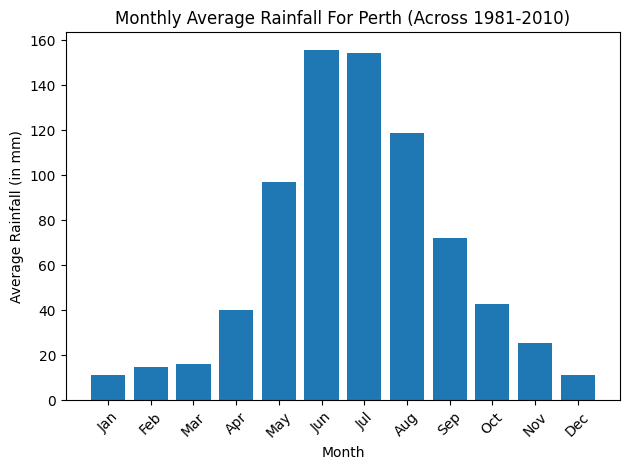
\includegraphics{Assignment-1_ICP_files/figure-pdf/cell-3-output-1.png}

\section{Problem 2(a) -
interpretation}\label{problem-2a---interpretation}

We can see from the chart that \textbf{June} is slightly higher in terms
of precipitation for the time slice of focus within the rainfall data
from the Perth Airport. However, it would have been July if I had not
included a `dropna' step in my code, which was done to ensure that the
next parts of the analysis would not suffer if I choose to use
statistical analyses that require all values to be present \& filled.

\begin{Shaded}
\begin{Highlighting}[]
\CommentTok{\# Problem 2(b) {-} Plotting July Rainfall trends}

\CommentTok{\# creating a July{-}specific dataset}
\NormalTok{perth\_july\_df }\OperatorTok{=}\NormalTok{ perth\_df[perth\_df[}\StringTok{\textquotesingle{}MONTH\textquotesingle{}}\NormalTok{] }\OperatorTok{==} \DecValTok{7}\NormalTok{]}

\CommentTok{\# plotting the July{-}only trendline}
\ImportTok{from}\NormalTok{ scipy.stats }\ImportTok{import}\NormalTok{ linregress}

\CommentTok{\# Calculate the trendline}
\NormalTok{slope, intercept, r\_value, p\_value, std\_err }\OperatorTok{=}\NormalTok{ linregress(perth\_july\_df[}\StringTok{\textquotesingle{}YEAR\textquotesingle{}}\NormalTok{], perth\_july\_df[}\StringTok{\textquotesingle{}PRCP\textquotesingle{}}\NormalTok{])}
\NormalTok{trendline }\OperatorTok{=}\NormalTok{ slope }\OperatorTok{*}\NormalTok{ perth\_july\_df[}\StringTok{\textquotesingle{}YEAR\textquotesingle{}}\NormalTok{] }\OperatorTok{+}\NormalTok{ intercept}

\CommentTok{\# Plot the trendline}
\NormalTok{plt.figure(figsize}\OperatorTok{=}\NormalTok{(}\DecValTok{10}\NormalTok{, }\DecValTok{6}\NormalTok{))}
\NormalTok{plt.scatter(perth\_july\_df[}\StringTok{\textquotesingle{}YEAR\textquotesingle{}}\NormalTok{], perth\_july\_df[}\StringTok{\textquotesingle{}PRCP\textquotesingle{}}\NormalTok{], label}\OperatorTok{=}\StringTok{\textquotesingle{}July Rainfall\textquotesingle{}}\NormalTok{)}
\NormalTok{plt.plot(perth\_july\_df[}\StringTok{\textquotesingle{}YEAR\textquotesingle{}}\NormalTok{], trendline, color}\OperatorTok{=}\StringTok{\textquotesingle{}red\textquotesingle{}}\NormalTok{, linestyle}\OperatorTok{=}\StringTok{\textquotesingle{}{-}{-}\textquotesingle{}}\NormalTok{, label}\OperatorTok{=}\SpecialStringTok{f\textquotesingle{}Trendline (y=}\SpecialCharTok{\{}\NormalTok{slope}\SpecialCharTok{:.2f\}}\SpecialStringTok{x + }\SpecialCharTok{\{}\NormalTok{intercept}\SpecialCharTok{:.2f\}}\SpecialStringTok{)\textquotesingle{}}\NormalTok{)}

\NormalTok{plt.xlabel(}\StringTok{"Year"}\NormalTok{)}
\NormalTok{plt.ylabel(}\StringTok{"Rainfall in July (in mm)"}\NormalTok{)}
\NormalTok{plt.title(}\StringTok{"July Rainfall in Perth (since 1944) with Trendline"}\NormalTok{)}
\NormalTok{plt.legend()}
\NormalTok{plt.grid(}\VariableTok{True}\NormalTok{)}
\NormalTok{plt.tight\_layout()}
\NormalTok{plt.show()}
\end{Highlighting}
\end{Shaded}

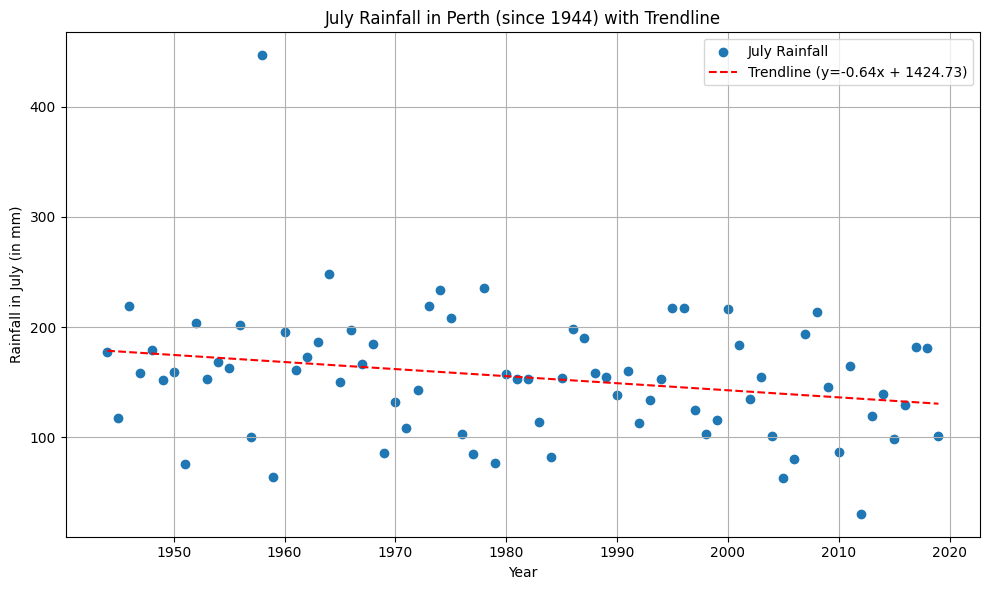
\includegraphics{Assignment-1_ICP_files/figure-pdf/cell-4-output-1.png}

\begin{Shaded}
\begin{Highlighting}[]
\CommentTok{\# Problem 2(b) {-} Plotting July Rainfall trends {-} Continued}
\CommentTok{\# exploring the early (1951 {-} 1980) and late (1981 {-} 2010) differences}

\CommentTok{\# setting the timeframes and slicing}
\NormalTok{early\_start\_date }\OperatorTok{=}\NormalTok{ pd.to\_datetime(}\StringTok{\textquotesingle{}1951{-}01{-}01\textquotesingle{}}\NormalTok{)}
\NormalTok{early\_end\_date }\OperatorTok{=}\NormalTok{ pd.to\_datetime(}\StringTok{\textquotesingle{}1980{-}12{-}31\textquotesingle{}}\NormalTok{)}
\NormalTok{late\_start\_date }\OperatorTok{=}\NormalTok{ pd.to\_datetime(}\StringTok{\textquotesingle{}1981{-}01{-}01\textquotesingle{}}\NormalTok{)}
\NormalTok{late\_end\_date }\OperatorTok{=}\NormalTok{ pd.to\_datetime(}\StringTok{\textquotesingle{}2011{-}01{-}01\textquotesingle{}}\NormalTok{)}

\NormalTok{early\_perth\_df }\OperatorTok{=}\NormalTok{ perth\_july\_df[(perth\_july\_df[}\StringTok{\textquotesingle{}DATE\textquotesingle{}}\NormalTok{] }\OperatorTok{\textgreater{}=}\NormalTok{ early\_start\_date) }\OperatorTok{\&}\NormalTok{ (perth\_july\_df[}\StringTok{\textquotesingle{}DATE\textquotesingle{}}\NormalTok{] }\OperatorTok{\textless{}=}\NormalTok{ early\_end\_date)]}
\NormalTok{late\_perth\_df }\OperatorTok{=}\NormalTok{ perth\_july\_df[(perth\_july\_df[}\StringTok{\textquotesingle{}DATE\textquotesingle{}}\NormalTok{] }\OperatorTok{\textgreater{}=}\NormalTok{ late\_start\_date) }\OperatorTok{\&}\NormalTok{ (perth\_july\_df[}\StringTok{\textquotesingle{}DATE\textquotesingle{}}\NormalTok{] }\OperatorTok{\textless{}=}\NormalTok{ late\_end\_date)]}

\CommentTok{\# statistical test here will be checking the different trend lines}
\NormalTok{e\_slope, e\_intercept, e\_r\_value, e\_p\_value, e\_std\_err }\OperatorTok{=}\NormalTok{ linregress(early\_perth\_df[}\StringTok{\textquotesingle{}YEAR\textquotesingle{}}\NormalTok{], early\_perth\_df[}\StringTok{\textquotesingle{}PRCP\textquotesingle{}}\NormalTok{])}
\NormalTok{e\_trendline }\OperatorTok{=}\NormalTok{ e\_slope }\OperatorTok{*}\NormalTok{ early\_perth\_df[}\StringTok{\textquotesingle{}YEAR\textquotesingle{}}\NormalTok{] }\OperatorTok{+}\NormalTok{ e\_intercept}

\NormalTok{l\_slope, l\_intercept, l\_r\_value, l\_p\_value, l\_std\_err }\OperatorTok{=}\NormalTok{ linregress(late\_perth\_df[}\StringTok{\textquotesingle{}YEAR\textquotesingle{}}\NormalTok{], late\_perth\_df[}\StringTok{\textquotesingle{}PRCP\textquotesingle{}}\NormalTok{])}
\NormalTok{l\_trendline }\OperatorTok{=}\NormalTok{ l\_slope }\OperatorTok{*}\NormalTok{ late\_perth\_df[}\StringTok{\textquotesingle{}YEAR\textquotesingle{}}\NormalTok{] }\OperatorTok{+}\NormalTok{ l\_intercept}

\CommentTok{\# printing our outputs for comparison}
\BuiltInTok{print}\NormalTok{(}\SpecialStringTok{f"}\CharTok{\textbackslash{}n}\SpecialStringTok{Early Trendline Equation: y = }\SpecialCharTok{\{}\NormalTok{e\_slope}\SpecialCharTok{:.2f\}}\SpecialStringTok{x + }\SpecialCharTok{\{}\NormalTok{e\_intercept}\SpecialCharTok{:.2f\}}\SpecialStringTok{"}\NormalTok{)}
\BuiltInTok{print}\NormalTok{(}\SpecialStringTok{f"R{-}squared value: }\SpecialCharTok{\{}\NormalTok{e\_r\_value}\OperatorTok{**}\DecValTok{2}\SpecialCharTok{:.2f\}}\SpecialStringTok{"}\NormalTok{)}
\BuiltInTok{print}\NormalTok{(}\SpecialStringTok{f"p{-}value: }\SpecialCharTok{\{}\NormalTok{e\_p\_value}\SpecialCharTok{\}}\SpecialStringTok{"}\NormalTok{)}
\BuiltInTok{print}\NormalTok{(}\SpecialStringTok{f"}\CharTok{\textbackslash{}n}\SpecialStringTok{Late Trendline Equation: y = }\SpecialCharTok{\{}\NormalTok{l\_slope}\SpecialCharTok{:.2f\}}\SpecialStringTok{x + }\SpecialCharTok{\{}\NormalTok{l\_intercept}\SpecialCharTok{:.2f\}}\SpecialStringTok{"}\NormalTok{)}
\BuiltInTok{print}\NormalTok{(}\SpecialStringTok{f"R{-}squared value: }\SpecialCharTok{\{}\NormalTok{l\_r\_value}\OperatorTok{**}\DecValTok{2}\SpecialCharTok{:.2f\}}\SpecialStringTok{"}\NormalTok{)}
\BuiltInTok{print}\NormalTok{(}\SpecialStringTok{f"p{-}value: }\SpecialCharTok{\{}\NormalTok{l\_p\_value}\SpecialCharTok{\}}\SpecialStringTok{"}\NormalTok{)}
\end{Highlighting}
\end{Shaded}

\begin{verbatim}

Early Trendline Equation: y = -0.94x + 2015.97
R-squared value: 0.01
p-value: 0.5557170847853263

Late Trendline Equation: y = -0.49x + 1129.55
R-squared value: 0.01
p-value: 0.601563230371377
\end{verbatim}

\section{2(b) - interpretation}\label{b---interpretation}

Looking at our output results, we can see that there is a steeper slope
for the earlier era (1951 - 1980) than for the later era (1981 - 2010),
which indicates that rainfall fell more steeply per year in July in the
older era of our Perth data. This might sound surprising given that
climate change has been accelerating since the early era and is becoming
more difficult towards the present era, however the earlier era also had
a much higher intercept, meaning that this simple statistical model
predicts that the history of the area had much better rainfall than the
more contemporary era.

For both analyses, the p-values did not indicate statistical
significance, likely due to the small nature of the sample size.
However, these trendlines are a good tool for us to consider as general
predictions, if we were seeking to get better statistical significance
we would expand to include neighbouring weatherstations to the Perth
Airport and generate a sample large enough to deliver a reasonable level
of meaning.

\begin{Shaded}
\begin{Highlighting}[]
\CommentTok{\# Problem 2(c) {-} grouping all winter rainfall}

\CommentTok{\# returning to our original df}
\NormalTok{winter\_months }\OperatorTok{=}\NormalTok{ [}\DecValTok{5}\NormalTok{,}\DecValTok{6}\NormalTok{,}\DecValTok{7}\NormalTok{,}\DecValTok{8}\NormalTok{] }\CommentTok{\# the MONTH column is in numerical format}
\NormalTok{winter\_perth\_df }\OperatorTok{=}\NormalTok{ perth\_df[perth\_df[}\StringTok{\textquotesingle{}MONTH\textquotesingle{}}\NormalTok{].isin(winter\_months)].copy()}

\CommentTok{\# creating our winter average}
\NormalTok{winter\_annual\_df }\OperatorTok{=}\NormalTok{ winter\_perth\_df.groupby(}\StringTok{\textquotesingle{}YEAR\textquotesingle{}}\NormalTok{)[}\StringTok{\textquotesingle{}PRCP\textquotesingle{}}\NormalTok{].mean().reset\_index()}
\NormalTok{winter\_annual\_df.rename(columns}\OperatorTok{=}\NormalTok{\{}\StringTok{\textquotesingle{}PRCP\textquotesingle{}}\NormalTok{: }\StringTok{\textquotesingle{}WINT\_AVG\_RAINFALL\textquotesingle{}}\NormalTok{\}, inplace}\OperatorTok{=} \VariableTok{True}\NormalTok{)}


\CommentTok{\# plotting the trendline}
\NormalTok{w\_slope, w\_intercept, w\_r\_value, w\_p\_value, w\_std\_err }\OperatorTok{=}\NormalTok{ linregress(winter\_annual\_df[}\StringTok{\textquotesingle{}YEAR\textquotesingle{}}\NormalTok{], winter\_annual\_df[}\StringTok{\textquotesingle{}WINT\_AVG\_RAINFALL\textquotesingle{}}\NormalTok{])}
\NormalTok{w\_trendline }\OperatorTok{=}\NormalTok{ w\_slope }\OperatorTok{*}\NormalTok{ winter\_annual\_df[}\StringTok{\textquotesingle{}YEAR\textquotesingle{}}\NormalTok{] }\OperatorTok{+}\NormalTok{ w\_intercept}

\CommentTok{\# assembling a scatterplot}
\NormalTok{plt.figure(figsize}\OperatorTok{=}\NormalTok{(}\DecValTok{12}\NormalTok{, }\DecValTok{6}\NormalTok{))}
\NormalTok{plt.scatter(winter\_annual\_df[}\StringTok{\textquotesingle{}YEAR\textquotesingle{}}\NormalTok{], winter\_annual\_df[}\StringTok{\textquotesingle{}WINT\_AVG\_RAINFALL\textquotesingle{}}\NormalTok{], label}\OperatorTok{=}\StringTok{\textquotesingle{}Average Winter Rainfall\textquotesingle{}}\NormalTok{)}
\NormalTok{plt.plot(winter\_annual\_df[}\StringTok{\textquotesingle{}YEAR\textquotesingle{}}\NormalTok{], w\_trendline, color}\OperatorTok{=}\StringTok{\textquotesingle{}red\textquotesingle{}}\NormalTok{, linestyle}\OperatorTok{=}\StringTok{\textquotesingle{}{-}{-}\textquotesingle{}}\NormalTok{, label}\OperatorTok{=}\SpecialStringTok{f\textquotesingle{}Trendline (y=}\SpecialCharTok{\{}\NormalTok{w\_slope}\SpecialCharTok{:.2f\}}\SpecialStringTok{x + }\SpecialCharTok{\{}\NormalTok{w\_intercept}\SpecialCharTok{:.2f\}}\SpecialStringTok{)\textquotesingle{}}\NormalTok{)}

\CommentTok{\# Add labels and title}
\NormalTok{plt.xlabel(}\StringTok{"Year"}\NormalTok{)}
\NormalTok{plt.ylabel(}\StringTok{"Average Rainfall for Winter (in mm)"}\NormalTok{)}
\NormalTok{plt.title(}\StringTok{"Average Winter (May {-} August) Rainfall in Perth Since 1944 with Trendline"}\NormalTok{)}
\NormalTok{plt.legend()}
\NormalTok{plt.grid(}\VariableTok{True}\NormalTok{)}
\NormalTok{plt.tight\_layout()}
\NormalTok{plt.show()}

\CommentTok{\# Checking our trendline}
\BuiltInTok{print}\NormalTok{(}\SpecialStringTok{f"}\CharTok{\textbackslash{}n}\SpecialStringTok{Trendline Equation: y = }\SpecialCharTok{\{}\NormalTok{w\_slope}\SpecialCharTok{:.2f\}}\SpecialStringTok{x + }\SpecialCharTok{\{}\NormalTok{w\_intercept}\SpecialCharTok{:.2f\}}\SpecialStringTok{"}\NormalTok{)}
\BuiltInTok{print}\NormalTok{(}\SpecialStringTok{f"R{-}squared value: }\SpecialCharTok{\{}\NormalTok{w\_r\_value}\OperatorTok{**}\DecValTok{2}\SpecialCharTok{:.2f\}}\SpecialStringTok{"}\NormalTok{)}
\BuiltInTok{print}\NormalTok{(}\SpecialStringTok{f"p{-}value: }\SpecialCharTok{\{}\NormalTok{w\_p\_value}\SpecialCharTok{\}}\SpecialStringTok{"}\NormalTok{)}
\end{Highlighting}
\end{Shaded}

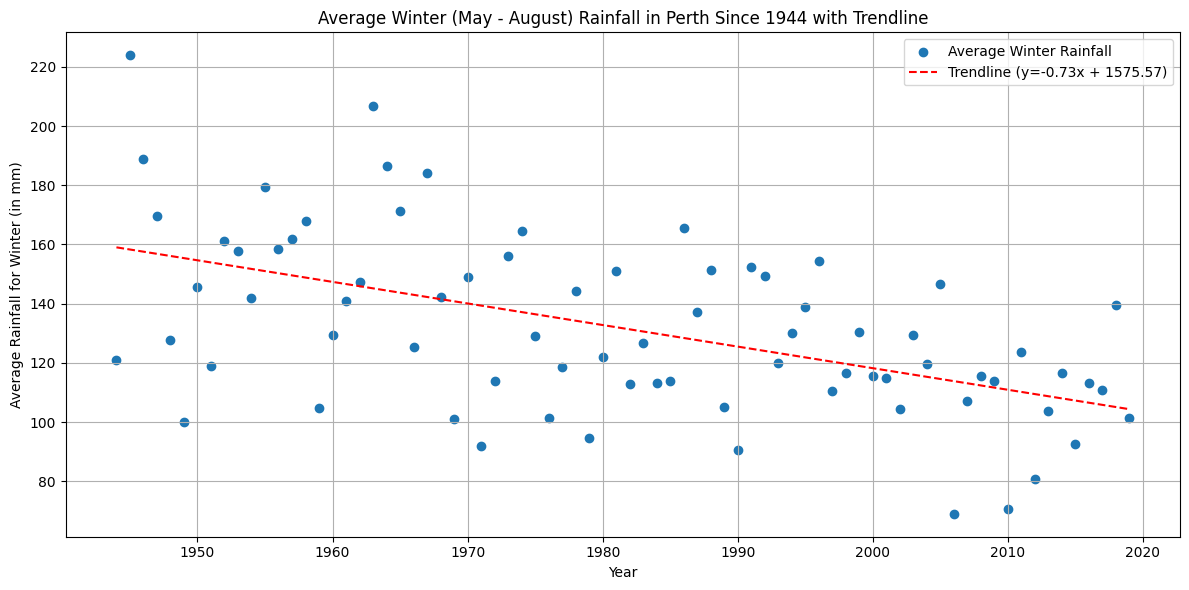
\includegraphics{Assignment-1_ICP_files/figure-pdf/cell-6-output-1.png}

\begin{verbatim}

Trendline Equation: y = -0.73x + 1575.57
R-squared value: 0.28
p-value: 6.998670645292783e-07
\end{verbatim}

\section{2(c) Interpretation}\label{c-interpretation}

The initial version of this scatter plot from just the July data showed
a fairly even scatter, however the inclusion of the winter seasonal
average has made the scatter trend more pronounced.

For my statistical test I looked at the trendline, which I copied into
the diagram here. This enhanced the scatter plot and makes it fairly
clear that the overall movement is downward in terms of rainfall, and
the R\textsuperscript{2} value of 0.28 shows that this trend explains a
fair amount of the variation in this dataset (with a p-value of
\textasciitilde7x10\textsuperscript{-7} so we can feel confident in the
statistical significance of these results). The earlier effort in
statistical modeling also generated slopes and R\textsuperscript{2}
values, however given that p-values were not statistically significant
and the R\textsuperscript{2} values were 0.01 for both the early half
and the later half of the data, this latest trendline with the average
winter season is statistically speaking more useful for furthering our
understanding responsibly.

\begin{Shaded}
\begin{Highlighting}[]
\CommentTok{\# 3(a) Histogram of temperature from 1981{-}2010}

\CommentTok{\# setting up for two plots together}
\NormalTok{fig, axes }\OperatorTok{=}\NormalTok{ plt.subplots(}\DecValTok{1}\NormalTok{, }\DecValTok{2}\NormalTok{, figsize}\OperatorTok{=}\NormalTok{(}\DecValTok{10}\NormalTok{, }\DecValTok{5}\NormalTok{))}

\CommentTok{\# Plot the first histogram in the first subplot}
\NormalTok{axes[}\DecValTok{0}\NormalTok{].hist(us\_temp\_df[}\StringTok{\textquotesingle{}normal\_1981\_2010\textquotesingle{}}\NormalTok{], bins}\OperatorTok{=}\DecValTok{30}\NormalTok{, color}\OperatorTok{=} \StringTok{\textquotesingle{}skyblue\textquotesingle{}}\NormalTok{, edgecolor}\OperatorTok{=} \StringTok{\textquotesingle{}black\textquotesingle{}}\NormalTok{)}
\NormalTok{axes[}\DecValTok{0}\NormalTok{].set\_title(}\StringTok{\textquotesingle{}1981{-}2010 County Temperatures\textquotesingle{}}\NormalTok{)}
\NormalTok{axes[}\DecValTok{0}\NormalTok{].set\_xlabel(}\StringTok{\textquotesingle{}Temp (C)\textquotesingle{}}\NormalTok{)}
\NormalTok{axes[}\DecValTok{0}\NormalTok{].set\_ylabel(}\StringTok{\textquotesingle{}Frequency\textquotesingle{}}\NormalTok{)}

\CommentTok{\# Plot the second histogram in the second subplot}
\NormalTok{axes[}\DecValTok{1}\NormalTok{].hist(us\_temp\_df[}\StringTok{\textquotesingle{}rcp85\_2080\_2099\textquotesingle{}}\NormalTok{], bins}\OperatorTok{=}\DecValTok{30}\NormalTok{, color}\OperatorTok{=} \StringTok{\textquotesingle{}salmon\textquotesingle{}}\NormalTok{, edgecolor}\OperatorTok{=} \StringTok{\textquotesingle{}black\textquotesingle{}}\NormalTok{)}
\NormalTok{axes[}\DecValTok{1}\NormalTok{].set\_title(}\StringTok{\textquotesingle{}2080{-}2099 Projected County Temperatures\textquotesingle{}}\NormalTok{)}
\NormalTok{axes[}\DecValTok{1}\NormalTok{].set\_xlabel(}\StringTok{\textquotesingle{}Temp (°C)\textquotesingle{}}\NormalTok{)}
\NormalTok{axes[}\DecValTok{1}\NormalTok{].set\_ylabel(}\StringTok{\textquotesingle{}Frequency\textquotesingle{}}\NormalTok{)}
\NormalTok{plt.tight\_layout()}
\NormalTok{plt.show()}
\end{Highlighting}
\end{Shaded}

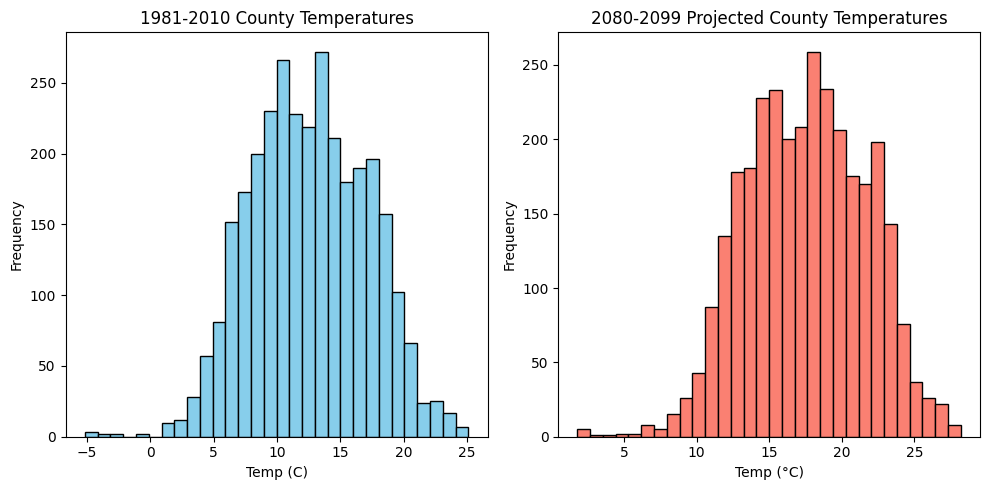
\includegraphics{Assignment-1_ICP_files/figure-pdf/cell-7-output-1.png}

\section{3(a) - interpretation}\label{a---interpretation}

As can be expected, the predicted temperatures in 2080-2099 show a
strong rightward shift towards climate extremes/increased annual average
temperatures. Interestingly, the distribution of counties in the
histogram retains a vague bell shaped distribution, which means we can
expect these predicting climate changes to be roughly evenly distributed
across US counties.

\begin{Shaded}
\begin{Highlighting}[]
\CommentTok{\# 3(b) Calculated Income Deciles}

\CommentTok{\# first, merging the data}
\NormalTok{us\_merged\_df }\OperatorTok{=}\NormalTok{ pd.merge(us\_temp\_df, us\_income\_df, left\_on}\OperatorTok{=} \StringTok{\textquotesingle{}fips\textquotesingle{}}\NormalTok{, right\_on}\OperatorTok{=} \StringTok{\textquotesingle{}fips\textquotesingle{}}\NormalTok{, how}\OperatorTok{=} \StringTok{\textquotesingle{}inner\textquotesingle{}}\NormalTok{)}

\CommentTok{\# next, creating our deciles for income}
\NormalTok{us\_merged\_df[}\StringTok{\textquotesingle{}income\_deciles\textquotesingle{}}\NormalTok{] }\OperatorTok{=}\NormalTok{ pd.qcut(us\_merged\_df[}\StringTok{\textquotesingle{}income\_per\_capita\_2018\textquotesingle{}}\NormalTok{], q}\OperatorTok{=} \DecValTok{10}\NormalTok{, labels}\OperatorTok{=} \VariableTok{False}\NormalTok{) }\OperatorTok{+} \DecValTok{1}

\CommentTok{\# next, grouping by our average temperatures for the time period}
\NormalTok{average\_temps\_df }\OperatorTok{=}\NormalTok{ us\_merged\_df.groupby([}\StringTok{\textquotesingle{}income\_deciles\textquotesingle{}}\NormalTok{])[[}\StringTok{\textquotesingle{}normal\_1981\_2010\textquotesingle{}}\NormalTok{,}\StringTok{\textquotesingle{}rcp85\_2020\_2039\textquotesingle{}}\NormalTok{, }\StringTok{\textquotesingle{}rcp85\_2040\_2059\textquotesingle{}}\NormalTok{, }\StringTok{\textquotesingle{}rcp85\_2080\_2099\textquotesingle{}}\NormalTok{]].mean().reset\_index()}

\BuiltInTok{print}\NormalTok{(average\_temps\_df)}
\end{Highlighting}
\end{Shaded}

\begin{verbatim}
   income_deciles  normal_1981_2010  rcp85_2020_2039  rcp85_2040_2059  \
0               1         15.358387        16.633868        17.691613   
1               2         14.776277        16.072329        17.146552   
2               3         14.035352        15.345230        16.438157   
3               4         13.123866        14.474455        15.595498   
4               5         12.707270        14.066774        15.180011   
5               6         11.979100        13.351000        14.496838   
6               7         11.394605        12.767488        13.907949   
7               8         10.901554        12.292372        13.458074   
8               9         10.237478        11.643873        12.826313   
9              10         10.980983        12.333084        13.454950   

   rcp85_2080_2099  
0        20.045851  
1        19.539103  
2        18.872312  
3        18.082923  
4        17.686174  
5        17.057449  
6        16.481029  
7        16.086495  
8        15.489746  
9        15.986360  
\end{verbatim}

\begin{Shaded}
\begin{Highlighting}[]
\CommentTok{\# 3(c) {-} Plotting Average temp for the selected timeslots}

\NormalTok{plt.figure(figsize}\OperatorTok{=}\NormalTok{(}\DecValTok{8}\NormalTok{, }\DecValTok{5}\NormalTok{))}
\NormalTok{plt.plot(average\_temps\_df[}\StringTok{\textquotesingle{}income\_deciles\textquotesingle{}}\NormalTok{], average\_temps\_df[}\StringTok{\textquotesingle{}normal\_1981\_2010\textquotesingle{}}\NormalTok{], marker}\OperatorTok{=}\StringTok{\textquotesingle{}o\textquotesingle{}}\NormalTok{, label}\OperatorTok{=}\StringTok{\textquotesingle{}Normal (1981{-}2010)\textquotesingle{}}\NormalTok{)}
\NormalTok{plt.plot(average\_temps\_df[}\StringTok{\textquotesingle{}income\_deciles\textquotesingle{}}\NormalTok{], average\_temps\_df[}\StringTok{\textquotesingle{}rcp85\_2080\_2099\textquotesingle{}}\NormalTok{], marker}\OperatorTok{=}\StringTok{\textquotesingle{}o\textquotesingle{}}\NormalTok{, label}\OperatorTok{=}\StringTok{\textquotesingle{}RCP8.5 (2080{-}2099)\textquotesingle{}}\NormalTok{)}

\CommentTok{\# plot design}
\NormalTok{plt.xlabel(}\StringTok{\textquotesingle{}Income Decile\textquotesingle{}}\NormalTok{)}
\NormalTok{plt.ylabel(}\StringTok{\textquotesingle{}Temperature (°C)\textquotesingle{}}\NormalTok{)}
\NormalTok{plt.title(}\StringTok{\textquotesingle{}Temperature (°C) vs. Income Decile\textquotesingle{}}\NormalTok{)}
\NormalTok{plt.xticks(average\_temps\_df[}\StringTok{\textquotesingle{}income\_deciles\textquotesingle{}}\NormalTok{]) }
\NormalTok{plt.legend()}
\NormalTok{plt.grid(}\VariableTok{True}\NormalTok{)}
\NormalTok{plt.tight\_layout()}
\NormalTok{plt.show()}
\end{Highlighting}
\end{Shaded}

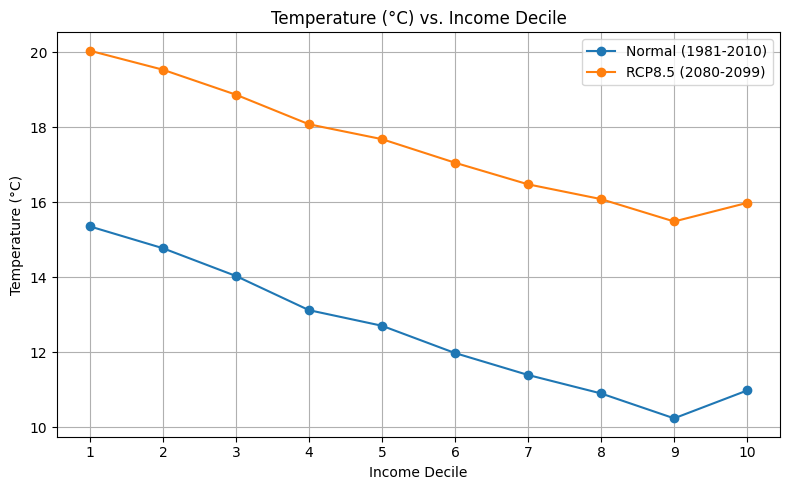
\includegraphics{Assignment-1_ICP_files/figure-pdf/cell-9-output-1.png}

\section{3 (d) - Interpretation}\label{d---interpretation}

I plotted both on the same chart to aide in the visual simplicity, I
understand that the prompt said ``plots'' but this way they are on the
same scale and nearby one another. In this way, we can see that we would
predict that the poorest American (counties) would be expected to
experience the hottest temperature under a changing climate scenario.
However, towards the extreme end of the income decile range we see a
slight uptick in the expected temperature in the RCP8.5 Scenario, with
this likely representing the increased shift in wealth towards
California and other Sunshine Belt states, whereas historically the
wealthiest Americans lived in the coldest parts (New York City, Boston,
Chicago).

\textbf{However}, this data set is only able to model based on the
currently available information, and it is quite likely that as climate
change becomes more extreme, the wealthiest Americans will be able to
afford to move away from the zones with dangerous temperature/flood
risk, so this is likely a poor predictor of future counties where wealth
will be concentrated, but it serves as a reasonable estimate for now.

\begin{Shaded}
\begin{Highlighting}[]
\CommentTok{\# 3(e) plotting our new variable}

\CommentTok{\# creating a new variable for the temperature change}
\NormalTok{us\_merged\_df[}\StringTok{\textquotesingle{}temp\_diff\textquotesingle{}}\NormalTok{] }\OperatorTok{=}\NormalTok{ us\_merged\_df[}\StringTok{\textquotesingle{}rcp85\_2080\_2099\textquotesingle{}}\NormalTok{] }\OperatorTok{{-}}\NormalTok{ us\_merged\_df[}\StringTok{\textquotesingle{}normal\_1981\_2010\textquotesingle{}}\NormalTok{]}

\CommentTok{\# Creating both a chropleth map (for clarity on part 2) and a histogram based on county data}

\CommentTok{\# choropleth map of temp change}
\NormalTok{us\_counties }\OperatorTok{=}\NormalTok{ geopandas.read\_file(}\StringTok{"counties.geojson"}\NormalTok{)}

\CommentTok{\# standardizing our fips codes}
\NormalTok{us\_counties[}\StringTok{\textquotesingle{}GEOID\textquotesingle{}}\NormalTok{] }\OperatorTok{=}\NormalTok{ us\_counties[}\StringTok{\textquotesingle{}GEOID\textquotesingle{}}\NormalTok{].astype(}\BuiltInTok{int}\NormalTok{)}
\NormalTok{us\_merged\_df[}\StringTok{\textquotesingle{}fips\textquotesingle{}}\NormalTok{] }\OperatorTok{=}\NormalTok{ us\_merged\_df[}\StringTok{\textquotesingle{}fips\textquotesingle{}}\NormalTok{].astype(}\BuiltInTok{int}\NormalTok{)}

\CommentTok{\# creating a merged dataframe for geospatial reference}
\NormalTok{merged\_gdf }\OperatorTok{=}\NormalTok{ us\_counties.merge(us\_merged\_df, left\_on}\OperatorTok{=}\StringTok{\textquotesingle{}GEOID\textquotesingle{}}\NormalTok{, right\_on}\OperatorTok{=}\StringTok{\textquotesingle{}fips\textquotesingle{}}\NormalTok{, how}\OperatorTok{=}\StringTok{\textquotesingle{}left\textquotesingle{}}\NormalTok{)}

\CommentTok{\# removing PR, AK, and HI to make the map reasonable}
\NormalTok{merged\_gdf }\OperatorTok{=}\NormalTok{ merged\_gdf[}\OperatorTok{\textasciitilde{}}\NormalTok{merged\_gdf[}\StringTok{\textquotesingle{}STATEFP\textquotesingle{}}\NormalTok{].isin([}\StringTok{\textquotesingle{}02\textquotesingle{}}\NormalTok{, }\StringTok{\textquotesingle{}15\textquotesingle{}}\NormalTok{, }\StringTok{\textquotesingle{}72\textquotesingle{}}\NormalTok{])]}

\CommentTok{\# plotting the choropleth}
\NormalTok{fig1, ax1 }\OperatorTok{=}\NormalTok{ plt.subplots(}\DecValTok{1}\NormalTok{, }\DecValTok{1}\NormalTok{, figsize}\OperatorTok{=}\NormalTok{(}\DecValTok{12}\NormalTok{, }\DecValTok{8}\NormalTok{))}
\NormalTok{merged\_gdf.plot(column}\OperatorTok{=}\StringTok{\textquotesingle{}temp\_diff\textquotesingle{}}\NormalTok{,}
\NormalTok{                cmap}\OperatorTok{=}\StringTok{\textquotesingle{}OrRd\textquotesingle{}}\NormalTok{,  }
\NormalTok{                linewidth}\OperatorTok{=} \FloatTok{0.2}\NormalTok{,}
\NormalTok{                ax}\OperatorTok{=}\NormalTok{ax1,}
\NormalTok{                edgecolor}\OperatorTok{=}\StringTok{\textquotesingle{}0.8\textquotesingle{}}\NormalTok{,}
\NormalTok{                legend}\OperatorTok{=}\VariableTok{True}\NormalTok{)}

\NormalTok{ax1.set\_title(}\StringTok{\textquotesingle{}Temperature Difference (°C) by County for 1981{-}2010 vs. 2080{-}2099 (contiguous USA)\textquotesingle{}}\NormalTok{)}


\CommentTok{\# Plot the histogram of income deciles}
\CommentTok{\# calculation step}
\NormalTok{avg\_temp\_diff\_by\_decile }\OperatorTok{=}\NormalTok{ merged\_gdf.groupby(}\StringTok{\textquotesingle{}income\_deciles\textquotesingle{}}\NormalTok{)[}\StringTok{\textquotesingle{}temp\_diff\textquotesingle{}}\NormalTok{].mean().reset\_index()}

\CommentTok{\# plotting step}
\NormalTok{fig2, ax2 }\OperatorTok{=}\NormalTok{ plt.subplots(}\DecValTok{1}\NormalTok{, }\DecValTok{1}\NormalTok{, figsize}\OperatorTok{=}\NormalTok{(}\DecValTok{8}\NormalTok{, }\DecValTok{6}\NormalTok{))}
\NormalTok{ax2.bar(avg\_temp\_diff\_by\_decile[}\StringTok{\textquotesingle{}income\_deciles\textquotesingle{}}\NormalTok{], avg\_temp\_diff\_by\_decile[}\StringTok{\textquotesingle{}temp\_diff\textquotesingle{}}\NormalTok{], color}\OperatorTok{=} \StringTok{\textquotesingle{}maroon\textquotesingle{}}\NormalTok{, edgecolor}\OperatorTok{=}\StringTok{\textquotesingle{}black\textquotesingle{}}\NormalTok{, alpha}\OperatorTok{=}\FloatTok{0.7}\NormalTok{) }\CommentTok{\# Bins represent temp\_diff}
\NormalTok{ax2.set\_title(}\StringTok{\textquotesingle{}Average Temperature Difference by Income Decile\textquotesingle{}}\NormalTok{) }
\NormalTok{ax2.set\_xlabel(}\StringTok{\textquotesingle{}Income Decile\textquotesingle{}}\NormalTok{)}
\NormalTok{ax2.set\_ylabel(}\StringTok{\textquotesingle{}Average Temperature Difference (°C)\textquotesingle{}}\NormalTok{)}

\NormalTok{plt.tight\_layout()}
\NormalTok{plt.show()}
\end{Highlighting}
\end{Shaded}

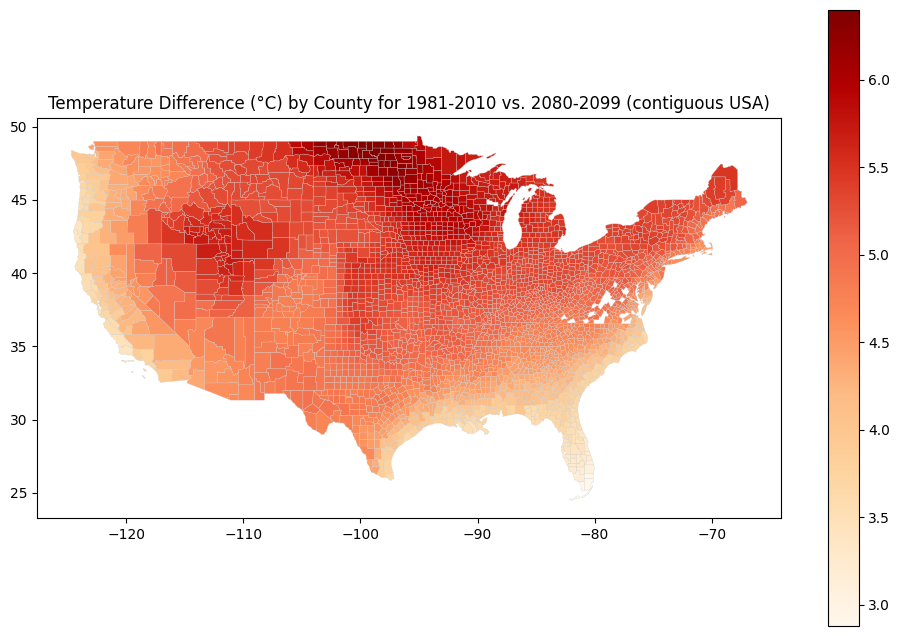
\includegraphics{Assignment-1_ICP_files/figure-pdf/cell-10-output-1.png}

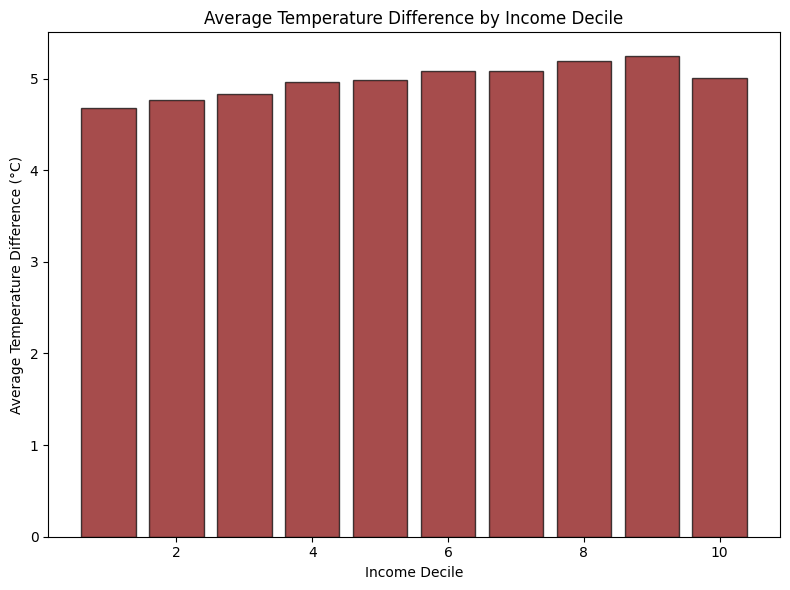
\includegraphics{Assignment-1_ICP_files/figure-pdf/cell-10-output-2.png}

\section{3(e) - Interpreting Our
Results}\label{e---interpreting-our-results}

In order to best interpret the spatial pattern of the results I decided
to do a little extra work and make a choropleth, which was absolutely
essential for me to understand what the data was showing. The map
clearly shows that there \textbf{will not} be even impacts from climate
change felt across the US, rather that there will be pockets in the
Mountain West and the Upper Midwest where the upwards temperature swing
will be more severe than the rest of the country. However, looking at
the average temperature change by decile (bar chart), we can see that
the changes will roughly impact across average income brackets evenly,
indeed with a slight bias towards the lower end of the socio-economic
spectrum recieving less impact from the changing climate. More likely
than not, this represents the areas of historic wealth distribution in
the United States, where cities like New York, Boston, Philly, and of
course Chicago are wealthier than major cities in Southern states, where
the upwards temperature change is predicted to be less severe. This data
would be improved by instead of tracking the migration patterns of
wealthy individuals as opposed to the locations that currently have high
incomes.

\section{3(f) - Exploring Policy
Ideas}\label{f---exploring-policy-ideas}

As a policy-maker, our goals in the face of climate change -- which
clearly per the choropleth map will be impacting the entire country --
should be unified around elevating \emph{all} people, with a
\emph{special emphasis on those whose livelihoods will be} \textbf{most}
\emph{disrupted by climate change}. There will certainly be disruptions
across many sectors, but in particular those reliant on
agricultural-sector careers will be impacted by the rising temps we see
here, so a better analysis we would want to run as policy makers here
would be to create a list of climate-vulnerable careers, pull data from
the American Community Survey, and create an index \emph{by county} that
shows us which counties are facing the greatest risk. Some jobs can be
relocated of course, but people are highly averse to moving from home
unless absolutely necessary, so it is far smarter as policy makers to
identify counties with the highest professional vulnerability and
connect those with members of Congress who represent the area and would
be motivated to engage in policy reform.

\begin{Shaded}
\begin{Highlighting}[]
\CommentTok{\# 3(g) {-}{-} Adding a new indicator}

\CommentTok{\# importing new data from the USDA {-} ERS}
\NormalTok{usda\_df }\OperatorTok{=}\NormalTok{ pd.read\_csv(}\StringTok{\textquotesingle{}2015CountyTypologyCodes.csv\textquotesingle{}}\NormalTok{)}
\NormalTok{usda\_df[}\StringTok{\textquotesingle{}FIPStxt\textquotesingle{}}\NormalTok{] }\OperatorTok{=}\NormalTok{ usda\_df[}\StringTok{\textquotesingle{}FIPStxt\textquotesingle{}}\NormalTok{].astype(}\BuiltInTok{int}\NormalTok{)}

\NormalTok{new\_merged\_gdf }\OperatorTok{=}\NormalTok{ merged\_gdf.merge(usda\_df, left\_on}\OperatorTok{=}\StringTok{\textquotesingle{}GEOID\textquotesingle{}}\NormalTok{, right\_on}\OperatorTok{=}\StringTok{\textquotesingle{}FIPStxt\textquotesingle{}}\NormalTok{, how}\OperatorTok{=}\StringTok{\textquotesingle{}left\textquotesingle{}}\NormalTok{)}


\CommentTok{\# creating the choropleth map with adjusted weights}
\NormalTok{fig, ax }\OperatorTok{=}\NormalTok{ plt.subplots(}\DecValTok{1}\NormalTok{, }\DecValTok{1}\NormalTok{)}
\NormalTok{new\_merged\_gdf.plot(}
\NormalTok{    column}\OperatorTok{=}\NormalTok{ new\_merged\_gdf[}\StringTok{\textquotesingle{}temp\_diff\textquotesingle{}}\NormalTok{] }\OperatorTok{*}\NormalTok{ (}\DecValTok{1} \OperatorTok{+}\NormalTok{ new\_merged\_gdf[}\StringTok{\textquotesingle{}Farming\_2015\_Update\textquotesingle{}}\NormalTok{]),}
\NormalTok{    cmap}\OperatorTok{=}\StringTok{\textquotesingle{}viridis\textquotesingle{}}\NormalTok{,}
\NormalTok{    linewidth}\OperatorTok{=}\FloatTok{0.2}\NormalTok{,}
\NormalTok{    ax}\OperatorTok{=}\NormalTok{ax,}
\NormalTok{    edgecolor}\OperatorTok{=}\StringTok{\textquotesingle{}0.8\textquotesingle{}}\NormalTok{,}
\NormalTok{    legend}\OperatorTok{=}\VariableTok{True}
\NormalTok{)}

\NormalTok{ax.set\_title(}\StringTok{\textquotesingle{}Choropleth Map Weighted for Farming{-}Dependent Counties\textquotesingle{}}\NormalTok{)}

\NormalTok{plt.show()}
\end{Highlighting}
\end{Shaded}

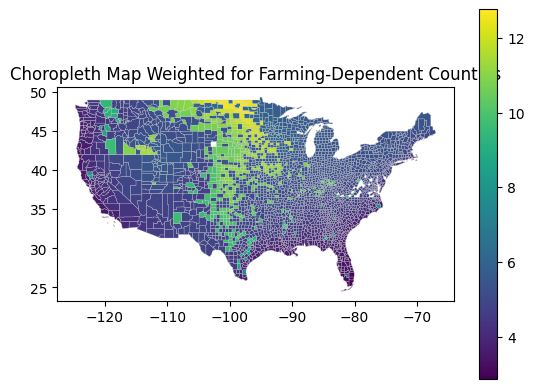
\includegraphics{Assignment-1_ICP_files/figure-pdf/cell-11-output-1.png}

\section{3(g) - Bonus! New Indicator}\label{g---bonus-new-indicator}

For this analysis, I felt that it would be best to adjust the choropleth
to color for the counties with the greatest degree of vulnerability to
climate risk, which I will define as farming-dependent counties that are
also high in terms of predicted temperature increase within the RCP 8.5
data. This new color scheme represents the relative social risk for
these counties that are dependent on climate sensitive industries

Data source:
\href{https://www.ers.usda.gov/data-products/county-typology-codes}{USDA
Economic Research Service}

\begin{Shaded}
\begin{Highlighting}[]
\CommentTok{\# 4 (a) Simple time series}
\CommentTok{\# fixing the data {-}{-} the conversion needs to split up the information}

\CommentTok{\# extracting year and month}
\KeywordTok{def}\NormalTok{ extract\_year\_month(year\_month):}
\NormalTok{    year }\OperatorTok{=} \BuiltInTok{int}\NormalTok{(}\BuiltInTok{str}\NormalTok{(year\_month)[:}\DecValTok{4}\NormalTok{])}
\NormalTok{    month }\OperatorTok{=} \BuiltInTok{int}\NormalTok{(}\BuiltInTok{str}\NormalTok{(year\_month)[}\DecValTok{4}\NormalTok{:])}
    \ControlFlowTok{return}\NormalTok{ year, month}

\CommentTok{\# splitting the time column into its components}
\NormalTok{gmst\_df[}\StringTok{\textquotesingle{}Year\_new\textquotesingle{}}\NormalTok{], gmst\_df[}\StringTok{\textquotesingle{}Month\textquotesingle{}}\NormalTok{] }\OperatorTok{=} \BuiltInTok{zip}\NormalTok{(}\OperatorTok{*}\NormalTok{gmst\_df[}\StringTok{\textquotesingle{}Year\textquotesingle{}}\NormalTok{].}\BuiltInTok{apply}\NormalTok{(extract\_year\_month))}
\NormalTok{gmst\_df[}\StringTok{\textquotesingle{}Year\_new\textquotesingle{}}\NormalTok{] }\OperatorTok{=}\NormalTok{ pd.to\_datetime(gmst\_df[}\StringTok{\textquotesingle{}Year\_new\textquotesingle{}}\NormalTok{], }\BuiltInTok{format}\OperatorTok{=}\StringTok{\textquotesingle{}\%Y\textquotesingle{}}\NormalTok{)}

\CommentTok{\# plotting the data correctly}
\NormalTok{plt.figure(figsize}\OperatorTok{=}\NormalTok{(}\DecValTok{12}\NormalTok{, }\DecValTok{8}\NormalTok{)) }
\NormalTok{plt.plot(gmst\_df[}\StringTok{\textquotesingle{}Year\_new\textquotesingle{}}\NormalTok{], gmst\_df[}\StringTok{\textquotesingle{}Anomaly\textquotesingle{}}\NormalTok{], marker}\OperatorTok{=} \StringTok{\textquotesingle{}o\textquotesingle{}}\NormalTok{, markersize}\OperatorTok{=} \DecValTok{3}\NormalTok{, linestyle}\OperatorTok{=}\StringTok{\textquotesingle{}{-}\textquotesingle{}}\NormalTok{, linewidth}\OperatorTok{=} \FloatTok{1.5}\NormalTok{, color}\OperatorTok{=}\StringTok{\textquotesingle{}lightgrey\textquotesingle{}}\NormalTok{)}
\NormalTok{plt.title(}\StringTok{\textquotesingle{}Time Series of Average Global Temperature Anomaly\textquotesingle{}}\NormalTok{)}
\NormalTok{plt.xlabel(}\StringTok{\textquotesingle{}Year\textquotesingle{}}\NormalTok{)}
\NormalTok{plt.ylabel(}\StringTok{\textquotesingle{}Average Global Temperature Anomaly (°C)\textquotesingle{}}\NormalTok{)}
\NormalTok{plt.grid(}\VariableTok{True}\NormalTok{)}
\NormalTok{plt.tight\_layout()}
\NormalTok{plt.show()}
\end{Highlighting}
\end{Shaded}

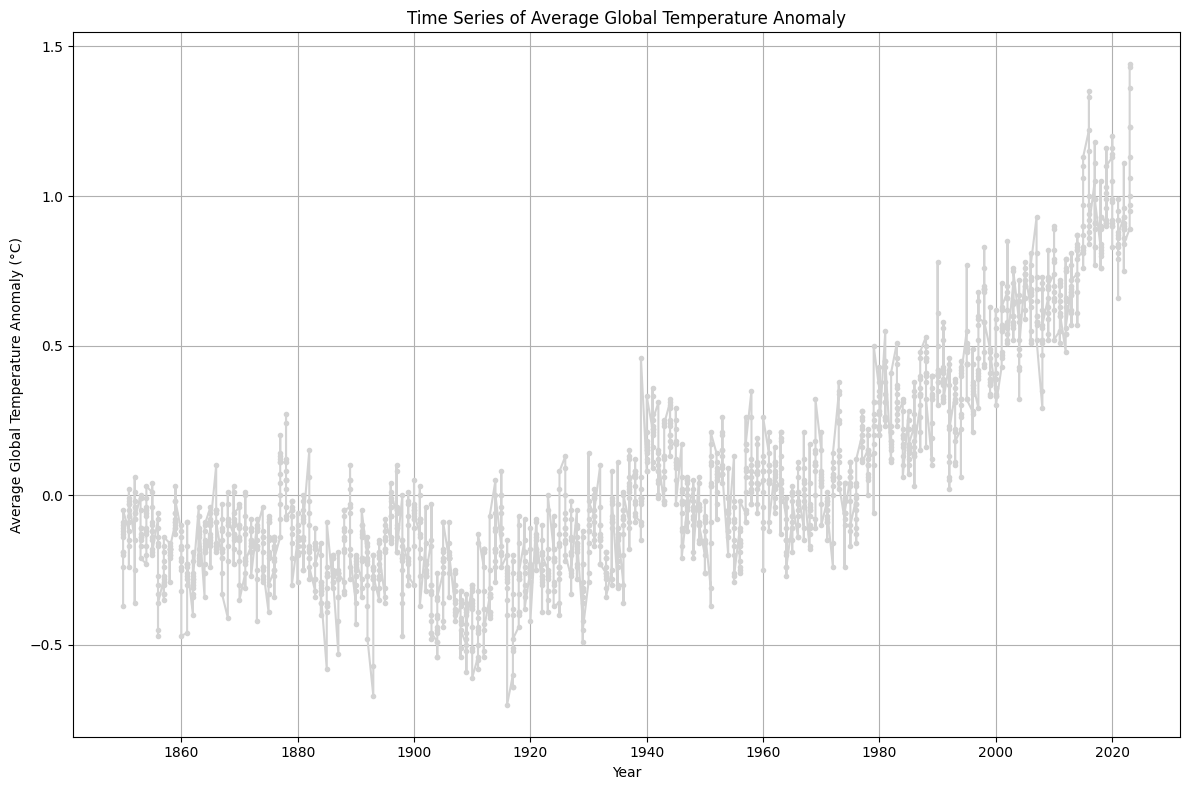
\includegraphics{Assignment-1_ICP_files/figure-pdf/cell-12-output-1.png}

\section{4(b) - Commentary on the chart generated in
4(a)}\label{b---commentary-on-the-chart-generated-in-4a}

There are a few key trends that are visible in the chart above:

\begin{itemize}
\item
  \textbf{Upward Acceleration the past 50 years}: Since the 1950s,
  following the end of WWII, we can see that a key element of the
  post-war world and rebuilding of Europe resulted in booming
  manufacturing, construction, and all manner of high-emissions
  activities that have continued to grow as population's have
  skyrocketed. Indeed in 1955 the world population was around 2.5
  billion, doubling by 1987 to 5 billion, and that upwards trend mirrors
  what we see in the chart above.
\item
  \textbf{Stable Varitaion from \textasciitilde1850 to 1900}: Despite
  this era containing some of the early days of the Industrial
  Revolution, this early era in the chart appears fairly flat/stable.
  There is of course some spikes and variation, but we can see that
  these early days of CO\textsubscript{2} emissions were still
  accumulating in the atmosphere and had not yet had a notable impact on
  the overall average climate. As the world exited the Little Ice Age, a
  period of generally cooler temps, it is reasonable to extrapolate that
  the CO\textsubscript{2} emissions stemming from Industrialization were
  yet to accumulate in the atmosphere enough to cause a consistent shift
  in the climate.
\item
  \textbf{Specific Incidents such as the Krakatoa Eruption of 1883 Can
  Be Spotted in This Data}: Another curiours trend we can observe in
  this chart are the effects of some specific planetary-disruptive
  activities, such as the spike downwards in global temperatures
  following the Krakatoa Eruption in 1883. This event released aerosols
  into the atmosphere at such high concentrations that it reduced the
  strength of sunlight on the Earth briefly (and also is a contributing
  factor to the rise of the Impressionist Art Movement). Additionally,
  global wars (WWI, WWII) can be seen impacting global temperature
  anomalies, likely due to the mass disruptions of economic activity,
  but looking closely at say the start of WWII in September of 1939, we
  can see that there is a global dip in the climate anomaly data.
\end{itemize}

\section{4(c) - Exploring alternative modeling
approaches}\label{c---exploring-alternative-modeling-approaches}

\textbf{The climate spiral} reminds me of when I try to play with a Hula
hoop and it gets increasingly harder and harder to maintain the same
smooth spinning! Joking aside, this format presents a compelling method
by which we can explain that the world's warming pattern is pulling
towards the extremes and that the process is rapidly devloving.
Linguistically, the term `spiraling' tends to be used to describe an
increasingly bad situation, so it gets bonus points in terms of
conveying the depth of the crisis. This visual does not do a good job of
conveying what the impacts of this would mean for an indvidual, whereas
the original time series showed to the reader that they could expect the
climate to be pushing upwards in terms of °C.

\textbf{The Climate Stripes} offer a simpler system than the climate
spiral, and indeed this type of simple color palatte speaks to the
average reader a lot more easily than do the other styles we have
discussed so far. First, this anchored relatively to the average
temperature from 1961 to 2010, which is a time period that the average
adult can actually remember, whereas the time-series and the spiral
compare to temperatures from the 1800's! Second, the colors in this are
much more pronounced than in the climate spiral, again making it easier
for the reader to see the distinction.

\section{4(d) - New Data Viz for Climate Change
Ideas:}\label{d---new-data-viz-for-climate-change-ideas}

Climate change data suffers from the scale not being one that an
individual can easily grasp, and my first suggestion would be to take
the most compelling of the models we have seen so far (the Climate
Stripes) and create a dashboard or similar dropdown menu that allows for
a person to look up their home (country, town, as granular as possible)
data to see \emph{how this has impacted them locally}. It is incredibly
hard to motivate people to take on global efforts like this if there
aren't easily tangible ways for them to conceptualize how harshly the
crisis is impacting them locally. To the extent that data for this
exists, having two parallel bars of climate stripes, one being global
and one being local, would be an excellent data visualization.

Thinking critically about the end users of these types of charts, we
know that climate change is of
\href{https://climatepromise.undp.org/news-and-stories/worlds-largest-survey-climate-change-out-heres-what-results-show}{global
concern}, however visualising in a relatable format to the broader
public is difficult, and one way I think this gap could be bridged is
framing the anomaly years as credit card debt. This is a fairly common
financial mechanism globally, and it provides a good intuitive
understanding as to why weather may be good (an individual month's
expenses in this metaphor), but the overall climate is a growing concern
(we are not paying off our balance and are accumulating runaway debt
because of the interest). The idea of a planetary `budget' for
CO\textsubscript{2} is one that I think could appeal because of it's
synergistic fit with this metaphor!




\end{document}
